%%%%%%%%%%%%%%%%%%%%%%%%%%%%%%%%%%%%%%%%%%%%%%%%%%%%%%%%%%%%%%%%%%%%%%%%%%%%%%%
%
% methodology
% Copyright (c) 2010 by tilo.mueller@rwth-aachen.de
% 
%%%%%%%%%%%%%%%%%%%%%%%%%%%%%%%%%%%%%%%%%%%%%%%%%%%%%%%%%%%%%%%%%%%%%%%%%%%%%%%

\chapter{Methodik}

Die Studie wurde als Online-Umfrage entwickelt, mit dem direkten Ziel die Forschungsfragen zu beantworten. Dazu wurden die Forschungsfragen und die zugehörigen Hypothesen aufgestellt und mit diesen Mitteln der Fragebogen erstellt.


\section{Konstrukte}
\label{sec:categories}
Um die Forschungsfragen sinnvoll zu beantworten wurden Konstrukte definiert, die Teilbereiche der Forschungsfrage abdecken sollen. Dabei wurde darauf geachtet, dass die Konstrukte gut auf die Forschungsfragen hinführen und durch Hypothesen aufeinander aufbauen können.
\begin{enumerate}
\item \label{itm:Kat0}\textbf{Nutzung von Google Diensten}: Das Nutzungsverhalten der Google Dienste von Seiten der Nutzer. Dieser Teil fragt vor allem allgemeine Daten zum Nutzungsverhalten ab. Darunter fallen unter anderem die Information, welche Dienste genutzt werden und wie viele Accounts die Nutzer haben.
\item \label{itm:Kat1}\textbf{Kenntnisse über Googles Datenschutz}: Angeeignetes Wissen über den Umgang mit personenbezogenen Daten bei Google, vor allem im Bezug auf die genutzten Dienste. Hierbei sind Fragen wie \glqq Bietet Google auf Nutzer zugeschnittene Werbung an?\grqq relevant.
\item \label{itm:Kat2}\textbf{Vertrauen in Google}: Das Glauben an auftretende negative Konsequenzen im Zusammenhang mit dem Preisgeben der Daten (vgl. Kim et al., 2008).
\item \label{itm:Kat3}\textbf{Wahrgenommenes Risiko für die Privatsphäre}: Das Glauben an auftretende negative Konsequenzen im Zusammenhang mit dem Preisgeben der Daten (vgl. Kim et al., 2008)
\item \label{itm:Kat4}\textbf{Bewusstsein über das Aufgeben der Privatsphäre}: Das Bewusstsein über den Verlust der Privatsphäre bei der Verwendung von Google Diensten.
\item \label{itm:Kat5}\textbf{Schutzmaßnahmen}: Verhalten des Nutzers zum Schutze der eigenen Privatsphäre
\end{enumerate}

\section{Hypothesen}
Nach der Entwicklung der Konstrukte wurden Hypothesen aufgestellt um diese zu verbinden und die Forschungsfragen zu beantworten.
\begin{description}
\item[\label{itm:H0}\textbf{H1}]Je aktiver eine Person Google nutzt, desto mehr Kenntnisse über Googles Datenschutz bekommt sie.
\item[\label{itm:H1}\textbf{H2}]Je mehr eine Person über Googles Datenschutz weiß, desto seltener gibt sie Teile ihrer Privatsphäre auf
\item[\label{itm:H2}\textbf{H3}]Je höher das Vertrauen in Google ist, desto geringer wird das Risiko eingeschätzt.
\item[\label{itm:H3}\textbf{H4}]Je höher das Risiko eingeschätzt wird, desto mehr Schutzmaßnahmen werden unternommen.
\item[\label{itm:H4}\textbf{H5}]Je mehr Schutzmaßnahmen eine Person verwendet, desto bewusster ist ihr das Aufgeben der Privatsphäre.
\end{description}

Durch die Umfrage sollen diese Hypothesen belegt oder widerlegt werden und somit die Zusammenhänge dargestellt und letzten Endes die Forschungsfrage beantwortet werden.

Der Zusammenhang zwischen den Kategorien und den Hypothesen soll anhand folgender Grafik verdeutlicht werden:
\begin{figure}[H]
\centering
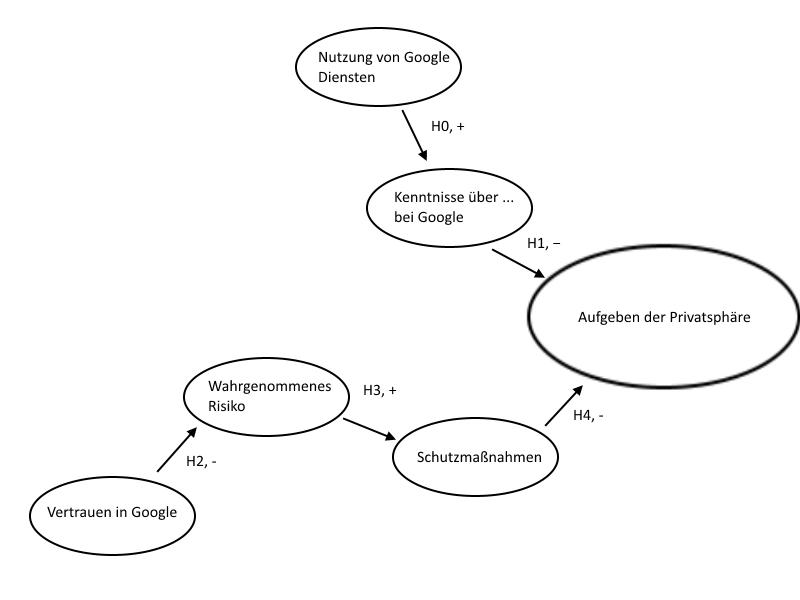
\includegraphics[scale=0.55]{images/bubbles}\\
\caption{Zusammenhang zwischen Kategorien und Hypothesen}\label{bubbles}
\end{figure}

\section{Fragebogenkonstruktion}
Zur Konstruktion des Fragebogens wurden die oben genannten Konstrukte und Hypothesen genommen um Fragen zu entwickeln. Diese Fragen sollten die Hypothesen möglichst gut beantworten und von Teilnehmern schnell und intuitiv lösbar sein. Das Ergebnis war eine Umfrage mit 39 Fragen, die in Seiten unterteilt waren, die ein schnelles und zielstrebiges durcharbeiten des Fragebogens vereinfachen sollte. 

Die Fragen sind zwar je einer der oben genannten Konstrukten zugeordnet, die Seiten in der Umfrage entsprechen aber nicht je einem Konstrukt. Dies hat den Zweck, dass Fragen die eventuell die Meinung der Teilnehmer beeinflussen könnten erst am Ende der Umfrage gestellt werden konnten.

Der letzte Teil der Umfrage ist eine Liste an demografischen Fragen die eine Einordnung der Teilnehmer erleichtern soll. Am Ende dieses Teiles steht noch eine Frage nach Feedback zur Umfrage.
Bei der Umfrageerstellung wurde auf eine Bearbeitungsdauer von 10-15 Minuten kalkuliert. Bei den ersten Testteilnehmern wurde als tatsächliche Bearbeitungsdauer ein durchschnittlicher Wert von 12 Minuten gemessen, was dem erwünschten Wert entsprochen hat.

Die folgenden Grafiken zeigen auf, wie die Verteilung der Fragen auf die in \ref{sec:categories} definierten Kategorien vorgenommen wurde und wie der Verlauf der Fragen in der Umfrage dargestellt wurde. Die Nummern der Fragen in der Grafik \ref{umldia} entsprechen den IDs der Fragen im Anhang (\ref{addendumquestions}ff). 

\begin{figure}[H]
\centering
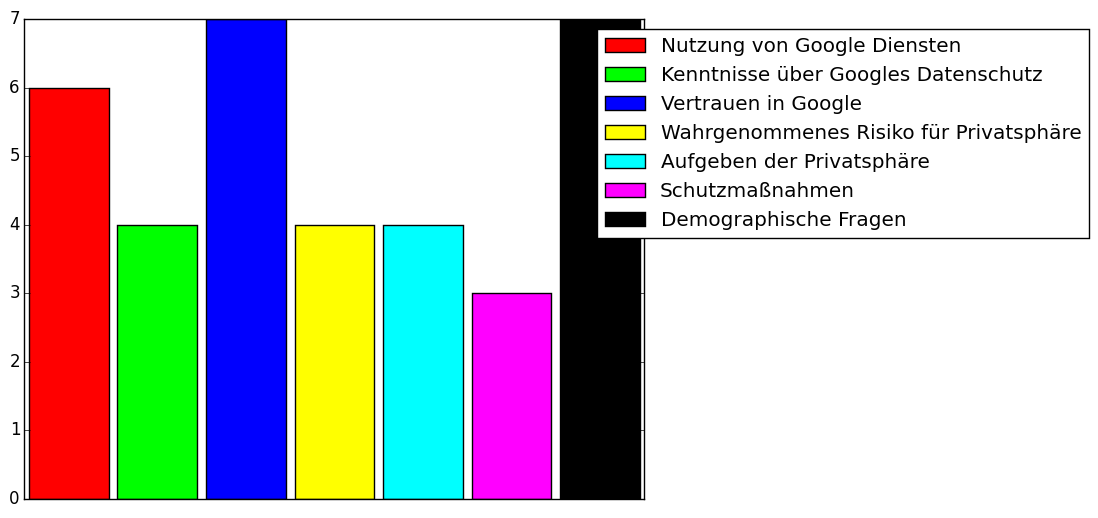
\includegraphics[width=\textwidth]{images/zahlenkategorien}\\
\caption{Anzahl der Fragen pro Kategorie in \ref{sec:categories}}\label{catnumbers}
\end{figure}

\begin{figure}[H]
\centering
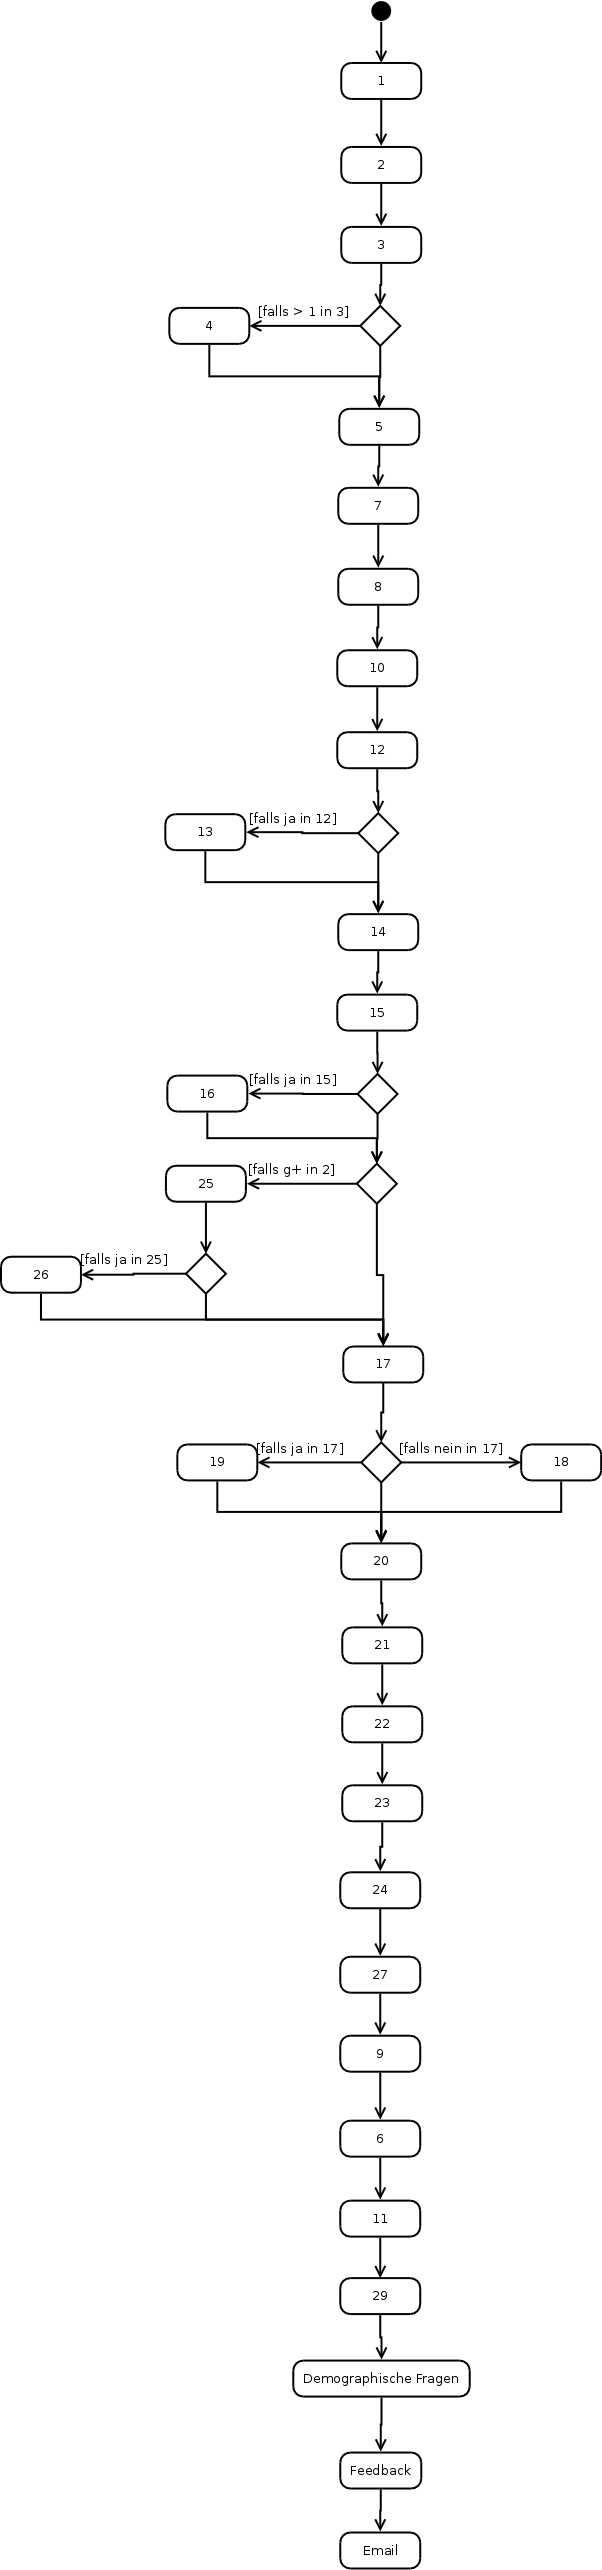
\includegraphics[height=\textheight]{images/umldia}\\
\caption{Anordnung der Fragen}\label{umldia}
\end{figure}


\section{Rekrutierung der Teilnehmer}
Die Umfrage wurde zuerst über Facebook und per Email über Familienmitglieder und Bekannte verteilt, mit der Angabe sie nach Möglichkeit auch weiter zu verteilen. Nachdem so schon eine relativ große Anzahl an Antworten erhalten wurden, wurde die Umfrage noch über den Email-Verteiler der Technischen Fakultät der Universität Erlangen-Nürnberg verbreitet.